\chapter{Design e training di una rete neurale con dati eterogenei in ingresso e risultati ottenuti}
\label{ch:MLP}
\section{Selezione di un sottinsieme completo del dataset}
I risultati ottenuti con la CNN possono essere migliorati o resi più attendibili con l'utilizzo
di altre tipologie di dati. Questi sono le informazioni relative al paziente al momento dell'arrivo in 
ospedale.
\\\\
Tali dati sono di vario tipo, quelli usati dal dataset considerato sono: 
\begin{itemize}
    \item Categorico, esprimono l'appartenenza ad una o più categorie
    \item Booleano, esprimo se il paziente è affetto da una certa patologia o presenta alcuni 
    \item Numerici
\end{itemize}
In questa fase è importante che tutti i dati siano presenti per ogni paziente. Per tale motivo si è dovuto 
trovare un sottinsieme del dataset che presenti il maggior numero di dati. 
\\\\
Per fare ciò sono state eliminate le colonne che non avevano corrispondenze 
tra i pazienti, ovvero erano vuote oppure presentavano dati solo per pochi pazienti.
Al fine di ottenere un risultato migliore sono state eliminati anche i pazienti che non presentavano dati per 
la maggiorparte delle colonne del dataset.
\\\\
Effettuata tale operazione, si è proceduto col creare un unico dataset ottenuto dall'unione 
di training set e test set. Per fare ciò le colonne presenti tra i due devono essere le stesse.
Per tale motivo si è giunti ad un dataset formato dalle seguenti colonne:
\begin{itemize}
    \item Ospedale, dato categorico che rappresenta l'ospedale che ha accolto il paziente tra A,B,C,D,E e F 
    \item Età, dato numerico
    \item Sesso, categorico binario, ovvero maschio o femmina
    \item Tosse, binario
    \item Difficoltà respiratorie
    \item Numero di cellule bianche, dato numerico che indica la percentuale di globuli bianchi nel sangue
    \item Pressione sanguigna alta,  binario
    \item Diabete, binario
    \item Demenza, binario 
    \item BPCO (Broncopneumopatia cronica ostruttiva), binario 
    \item Cancro, binario 
    \item Malattia renale cronica, binario
\end{itemize}
Tali dati sono presenti per 946 pazienti del training set e 472 del test set, per cui abbiamo un dataset di 1218 pazienti.
Questo dataset sarà poi suddiviso in training, validation e test set, per effettuare l'allenamento della rete e per verificare la capacità di effettuare previsioni.
$\\\\$
\begin{tcolorbox}[tab2,tabularx={Y|Y|Y|Y|Y|Y|Y|Y|Y|Y},title=\text{Estratto del dataset dato dall'unione dei due di partenza},width=\textwidth, center=\textwidth]
    \centering
    \begin{tabular}{l|c|c|c|c|c|c|c|l}
        ImageFile & H. & Age & .... & Cough & WBC & Ic. & H.B.P. & Prognosis \\ \hline \hline
        ... & ... & ... & ... & ... & ... & ... & ... & ...\\
        P\_281.png & E & 68 &...  & 0 & 7.33  & 0 & 1 &  MILD   \\
        P\_544.png & F & 72 &...  & 0 & 9.6  & 0 & 1 &  SEVERE   \\
        P\_657.png & C & 83 & ... & 1 & 9 & 0 & 1 &  SEVERE   \\
        P\_1\_93.png & F & 66 & ... & 0 & 10 & 0 & 0 & SEVERE   \\
        P\_73.png & A & 48 & ...  & 1 & 9.13 & 0 & 0  & MILD  \\
        ... & ... & ... & ... & ... & ... & ... & ... & ...
    \end{tabular}     
\end{tcolorbox}
$\\\\$
Ora che si presenta il dataset completo, si procede col trasformare tutti i dati nello stesso formato, ovvero in valori binari \cite{ar}.
Partendo dai dati categorici, si procede usando la codifica one-hot. Tale procedura prevede che le categorie relative al dato vengano 
trasformate in una rappresentazione binaria, in cui ogni categoria è rappresentata da una serie di zeri ed un unico uno presente nella categoria
codificata.
Per quanto riguarda il sesso, essendo una categoria binaria, si può usare un valore binario, per cui un sesso sarà rappresentato da 0 e l'altro da 1.
L'ospedale è un dato che prevede sei categorie, per cui queste saranno rappresentate da sei bit. Ogni rappresentazione
presenterà cinque zeri ed un unico uno (es. 001000).
\\\\
A livello pratico tali trasfromazioni sono state implementate usando la libreria scikit-learn, in particolare le funzioni
MultiLabelBinarizer(), per l'ospedale, e LabelBinarizer() per il sesso. In tal modo si riesce a trasformare le categorie in array di 
bit, ovvero valori compresi in [0,1].
\\\\
Per gestire i valori numerici si sfrutta un'altra funzione di scikit-learn, ovvero MinMaxScaler().
Tale funzione scala i valori dati in input in un range specificato, nel caso in considerazione [0,1].
La trasformazione avviene mediante:
\begin{equation*}
    \begin{array}{l}
        X_{std} = \dfrac{(X - X.min(axis=0))}  {(X.max(axis=0) - X.min(axis=0))} \\\\
        X_{scaled} = X_{std} * (max - min) + min
    \end{array}
\end{equation*}
\\\\
I valori binari infine sono rimasti invariati, poiché esprimono il valore nel range desiderato.

\section{Struttura percettrone multistrato}

Avendo ora convertito i dati del dataset in modo da essere in [0,1], si può iniziare a costruire la rete che deve fare previsioni 
prendendo come input tali dati. 
È importante notare che una volta effettuata la codifica one-hot della colonna relativa all'ospedale, si ottiene un vettore di dimensione 6 (una per ogni categoria) al 
posto dell'unica colonna che rappresenta il dato. Per tale motivo la dimensione dell'input della rete non è 
più 12 (in base al numero di colonne presenti inizialmente), ma 17.
\\\\
La rete dunque sarà formata da due layer:
\begin{itemize}
    \item un Dense() layer formato da 30 neuroni
    \item un Dense() layer formato da 5 neuroni
\end{itemize}
Il primo layer è colui che si occupa di ricevere anche gli input, per cui la dimensione degli input dovrà essere pari a 17.
Il secondo layer, invece, è formato da soli 5 layer e si occupa di effettuare una prima classificazione.
Entrambi i layer presentano come funzione di attivazione ReLu.
\\\\
Con tale rete, si riesce dunque ad effettuare il training relativo all'uso dei metadati.

\section{Creazione rete composta}
Per poter usare contemporaneamente le due reti neurali create, ovvero la CNN e la MLP, si necessita di 
un ulteriore passaggio.
Lo scopo di tale passaggio è avere una rete che accetti come input sia immagini che i metadati relativi, al fine
di ottenere una previsione più affidabile, poiché basata sull'uso di più dati.
\\\\
Per gestire gli output delle due reti questi vengono concatenati, in modo da ottenere un unico array di output.
Al fine di effettuare le predizioni su tale output si aggiunge, alla fine della rete, un ulteriore 
Dense layer, formato da un unico neurone, con funzione di attivazione Sigmoid e che prende un input della 
dimensione della combinazione degli output delle due reti. 
\\\\
Si può, infine, creare la rete che prende in input la combinazione degli input della rete, mentre l'output sarà determinato
dal nuovo layer inserito.
\begin{figure}[hp]
    \centering
        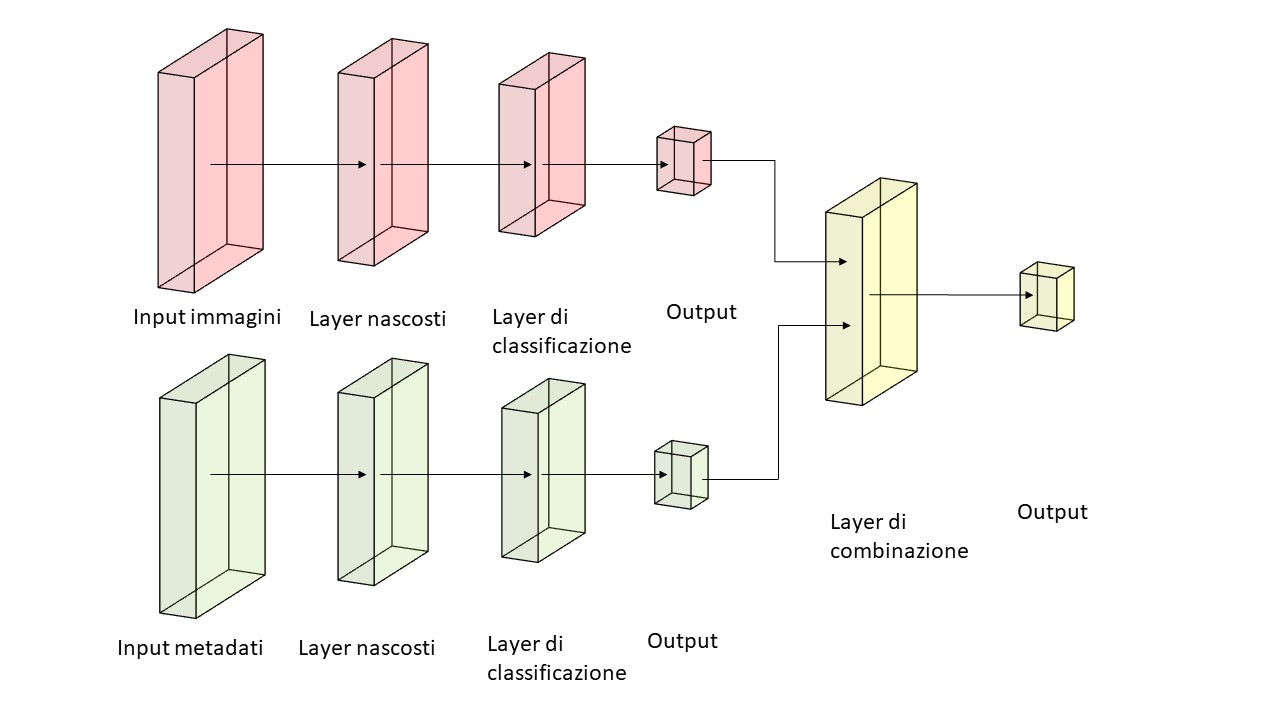
\includegraphics[width=12cm]{combined_meglio.jpg}  
        \caption{Rappresentazione della rete finale composta da CNN e MLP}
        %\label{SUBFIGURE LABEL 3}
\end{figure}
$\\$
Nella figura precedente sono riportate schematicamente la CNN (in rosso) e la MLP (in verde), le quali, una volta
combinate, creano la rete finale. L'output è dato dunque dalla composizione degli output.
I primi layer rappresentano la gestione degli input da parte delle rispettive reti, mentre i layer nascosti 
servono per svolgere varie funzionalità al fine di arrivare nei layer di classificazione avendo i dati delle 
dimensioni opportune. Infine vengono restituiti gli output che saranno combinati per produrre la previsione finale.
\section{Risultati dei test effettuati per la rete composta}
Ora si può dunque procedere con la compilazione della rete e con il training. I training sono stati effettuati usando i parametri usati 
nel caso della rete convoluzionale. 

\begin{figure}[htp]
    \centering
    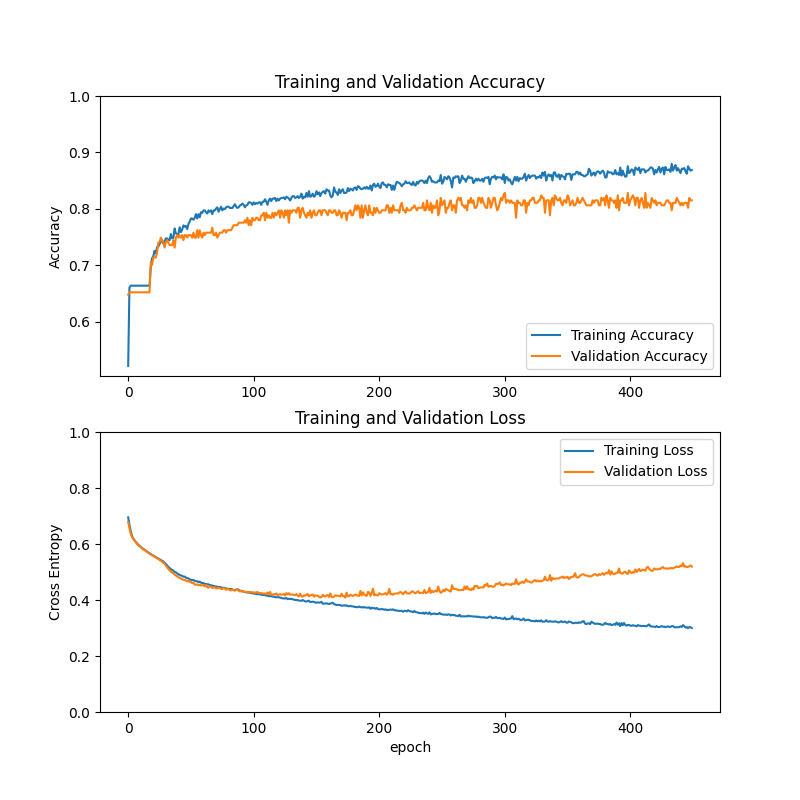
\includegraphics[width=\textwidth]{10_3_clin_giusto.png}
    \label{ 10^{-3} c }
    \caption{Test effettuato usando come learning rate $10^{-3}$}
\end{figure}

\begin{figure}[htp]
    \centering
    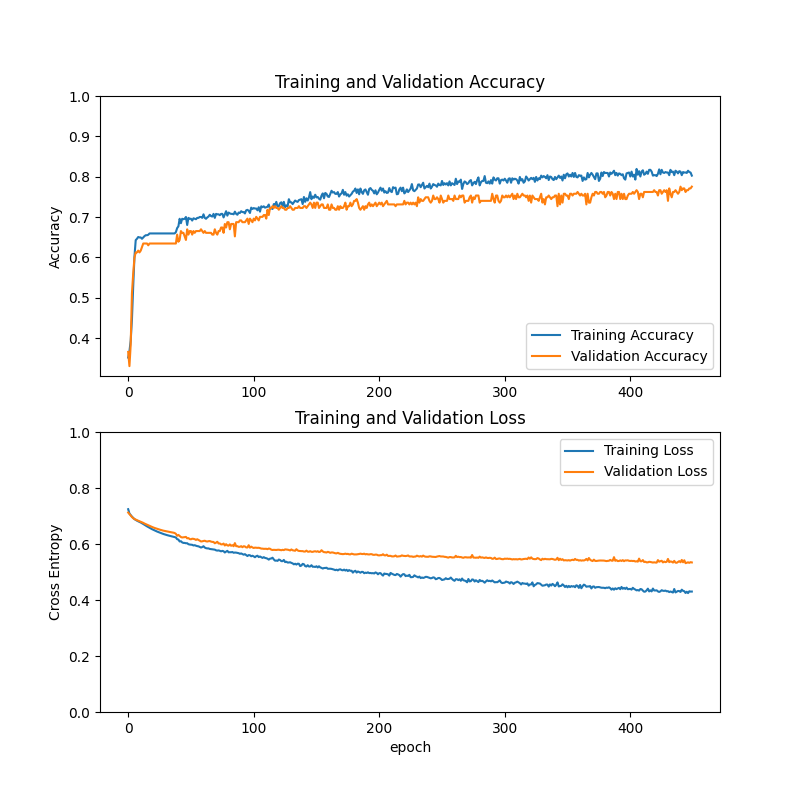
\includegraphics[width=\textwidth]{10_4_clin_giusto.png}
    \label{10^{-4} c}
    \caption{Test effettuato usando come learning rate $10^{-4}$}
\end{figure}
$\\\\$
Dai precedenti grafici si nota il corretto funzionamento suggerito dall'andamento decrescente della training loss.
Oltre a ciò è possibile notare un importante aumento della validatino accuracy rispetto a ciò che si era ottenuto nel caso 
di training con sole immagini. Infine si può notare come il learning rate pari a $10^{-3}$ sia anche in questo caso 
più performante.
\section{Confronto tra le varie reti adoperate nel progetto di tesi}

\begin{tcolorbox}[tab1,title=\text{Confronto dei risultati ottenuti con le varie reti usate}]
    \centering
    \begin{tabular}{l|c|c|c|l}
        Nome & accuracy & epoche & l.r. & descrizione \\ \hline \hline
        \makecell{CNN \\ t.l.}  &   55\%   &  150   & $10^{-3}$     & \makecell{rete neurale convoluzionale \\ transfer learning \\ con learning rate \\ pari a $10^{-3}$ (pagina \pageref{ 10^{-3} tl})} \\ \hline
        \makecell{CNN \\ t.l.}  &   53\%   &  150   & $10^{-4}$     & \makecell{rete neurale convoluzionale \\ transfer learning \\ con learning rate \\ pari a $10^{-4}$ (pagina \pageref{10^{-4} tl})} \\ \hline
        \makecell{CNN \\ f.t.}  &   60\%   &  150+30& $10^{-3}$     & \makecell{rete neurale convoluzionale \\ fine tuning \\ con learning rate \\ pari a $10^{-3}$ (pagina \pageref{ 10^{-3} ft})} \\ \hline
        \makecell{CNN \\ f.t.}  &   55\%   &  150+30& $10^{-4}$     & \makecell{rete neurale convoluzionale \\ fine tuning \\ con learning rate \\ pari a $10^{-4}$ (pagina \pageref{10^{-4} ft})}\\ \hline
        \makecell{CNN \\ d.a.}  &   63\%   &  150+500& $10^{-3}$     & \makecell{rete neurale convoluzionale \\ data augmentation \\ con learning rate \\ pari a $10^{-3}$ (pagina \pageref{Training Augmentation 1})}\\ \hline
        \makecell{CNN \\ d.a.}  &   57\%   &  150+500& $10^{-4}$     & \makecell{rete neurale convoluzionale \\ data augmentation \\ con learning rate \\ pari a $10^{-4}$ (pagina \pageref{Training Augmentation 2})}\\ \hline
        Composta  &   82\%     &   450  & $10^{-3}$     & \makecell{rete neurale convoluzionale \\ concatenato al percettrone \\con learning rate \\ pari a $10^{-3}$ (pagina \pageref{ 10^{-3} c })}\\ \hline
        Composta  &   79\%     &   450  & $10^{-4}$     & \makecell{rete neurale convoluzionale \\ concatenato al percettrone \\con learning rate \\ pari a $10^{-3}$ (pagina \pageref{10^{-4} c})}\\ 
    \end{tabular}     
\end{tcolorbox}
\newpage
$\\\\$
La tabella sopra riportata mostra un confronto tra le varie reti usate, le epoche dell'allenamento, il valore 
del learning rate e la validation accuracy ottenuta.
\\\\
Per quanto concerne le CNN con fine tuning sono state considerate anche le epoche precedenti relative al transfer learning.
In maniera analoga per la rete con data augmentation sono evidenziate le epoche relative al transfer learning e 
quelle relative al fine tuning.
\\\\ 
Da tale tabella si evince come, nonostante le varie tecniche usate per migliorare la precisione della CNN, l'uso 
di dati eterogenei comporta un netto miglioramento, dunque la combinazione di CNN e percettrone risulta essere 
la scelta ottimale per ottenere risultati più precisi